% outline

% requirements: suo apt install python3-pygments

% Intro
% Brief history
% Why?
% goto with settrace
% goto with bytecodes
% Crashing python with bytescodes
% Problems...
% Performance!

\documentclass{beamer}
\usepackage{minted}
\usetheme{default}
\hypersetup{colorlinks=true}
\usepackage{framed}
\usepackage[normalem]{ulem}
\usepackage{color}
\usepackage{graphicx}
\usepackage{hyperref}

\title{Recreating \texttt{goto} in Python; how and why}
\subtitle{CITRENZ 2023 Auckland}
\author{\texorpdfstring{Carl Cerecke\newline\url{carl.cerecke@nmit.ac.nz}}{Carl Cerecke}}
%\address{carl\@free.org.nz}
\institute{https://github.com/cdjc/goto}
\date{September 27--29, 2023}

\begin{document}

\begin{frame}[plain]
    \titlepage
\end{frame}

%\begin{frame}[fragile]{BASIC on the Commodore 64}
%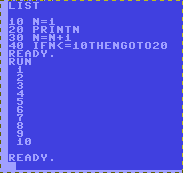
\includegraphics{c64.png}
%\end{frame}

\begin{frame}{Outline}
\begin{itemize}
    \item Memories
    \item Motivation
    \item Mechanism
    \item Measurement
    \item Musing
\end{itemize}

\end{frame}

\begin{frame}{Memories: A short history of goto}

\begin{itemize}
\item In the beginning was the \texttt{goto}
\item 1958 Heinz Zemanek expresses doubts about goto at pre-ALGOL meeting.
\item 1968 Edsgar Dijkstra ``GOTO Considered Harmful''
\item 1974 Don Knuth ``Structured Programming with go to statements''
\item 1987 Frank Rubin `` `GOTO Considered Harmful' Considered Harmful''
\item 1995 Java first major language with no \texttt{goto} statement.
\end{itemize}

\end{frame}

\begin{frame}{Motivation: Why add goto to Python?}

It seemed like a good idea at the time...
\vspace{1cm}

Also useful for:
\begin{enumerate}
\item Translating goto-filled code to python
\item Finite state machines
\item Generating python code programmatically
\item Breaking out of a nested loop
\end{enumerate}

\end{frame}
%
%\begin{frame}{Control flow in 1970's BASIC}
%\begin{itemize}
%    \item \texttt{if} statements have no \texttt{else}
%    \item No \texttt{while} loops. Only primitve \texttt{for} loopd
%    \item No functions. Only \texttt{GOSUB}
%    \item No scopes. Only global
%    \item Single-letter variable names
%\end{itemize}
%
%\end{frame}

\begin{frame}[fragile]{Motivation: An extract from \texttt{Hamurabi.bas} (1970's)}

From David Ahl's \emph{101 Basic Computer Games}, 1973

\vspace{1cm}

\begin{minted}[escapeinside=||]{basic}
320 PRINT "HOW MANY ACRES DO YOU WISH TO BUY";
321 INPUT Q: IF Q<0 THEN 850
322 IF Y*Q<=S THEN 330
323 GOSUB 710
324 GOTO 320
330 IF Q=0 THEN 340
331 A=A+Q: S=S-Y*Q: C=0
334 GOTO 400
\end{minted}

\end{frame}

\begin{frame}{Motivation: State Machines}
    \begin{itemize}
    \item A finite set of states. Transitions from one state to another on some input/event.
    \item Can model real world mechanisms: (Traffic lights, doors, game AI, etc.)
%    \item Equivalent in power to regular expressions.
%    \item Also \emph{Pushdown Automata} (a state machine with a stack). Used for parsing.
    \end{itemize}

    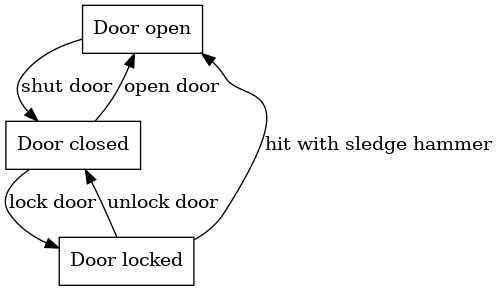
\includegraphics[scale=0.5]{doors.dot.png}
\end{frame}
%
%\begin{frame}{But it's already been done before!}
%
%\begin{itemize}
%\item April 1 2004, \href{http://entrian/goto}{http://entrian/goto}
%
%\item Uses \texttt{sys.settrace}
%
%\item Checks before the execution of \emph{every line} for goto. Slow
%
%\item Module scope, not function scope.
%\end{itemize}
%\end{frame}

\begin{frame}[fragile]{Mechanism: Goto using bytecode manipulation}
%
%\begin{itemize}
%\item Python source code is compiled into python \emph{bytecode} instructions.
%\item Byte codes have relative gotos: \texttt{JUMP\_FORWARD delta}
%\end{itemize}
    Within a function that uses gotos:

\begin{enumerate}
    \item (Mis)use attribute access for labels and goto.\\ e.g. \texttt{label .found}
    \item Extract a function's bytecode
    \item Replace bytecode for \texttt{goto .found} with relative jump to label
    \item Check for/Avoid/Mitigate various Bad Things
    \item Replace the function's bytecode with the new goto-ified bytecode
\end{enumerate}
%\item
%\item Each bytecode instruction is 2 bytes long.
%\item Python bytecodes have relative goto:
%
%\begin{itemize}
%\item JUMP\_FORWARD(delta)
%\item JUMP\_BACKWARD(delta)
%\end{itemize}
%\item CPython only.
%\item See the \verb!dis! module.
%\end{itemize}
\end{frame}

\begin{frame}[fragile]{Mechanism: Simple example function}



\begin{minted}{python}
from goto import goto

@goto       # the goto decorator rewrites bytecode
def find_value(rectangle, n):
    for line in rectangle:
        for value in line:
            if value == n:
                rval = "found
                goto .found   # jump down to label
    rval = "not found"
    label .found              # a no-op at runtime
    # ... other code here ...
    return rval
\end{minted}

%We can see python bytecodes:
%
%\begin{minted}{python}
%import dis
%dis.dis(fn)      # pretty print byte code
%\end{minted}

\end{frame}
%
%\begin{frame}[fragile]{Disassembly of simple function (without goto decorator)}
%\begin{tabular}{l|r|l|r|l}
%line & addr & opcode & par & interpretation \\
%\hline
%302 &          0 & LOAD\_GLOBAL         &     0 & (goto)  \\
%     &           3 &  LOAD\_ATTR               &   1  & (skip)  \\
%      &          6 &  POP\_TOP      &  &           \\
%\hline
%303   &          7 &  LOAD\_GLOBAL         &       2  & (print)  \\
%          &     10 &  LOAD\_FAST           &       0 &  (n)  \\
%              & 13 &  CALL\_FUNCTION        &      1  & (1 positional, 0 keyword pair)  \\
%     &          16 &  POP\_TOP            &     &  \\
%\hline
%304   &         17 &  LOAD\_GLOBAL        &        3  & (label)  \\
%     &          20 &  LOAD\_ATTR          &        1  & (skip)  \\
%     &          23 &  POP\_TOP            &     &  \\
%\hline
%     &          24 &  LOAD\_CONST         &        0  & (None)  \\
%     &          27 &  RETURN\_VALUE      &      &  \\
%\end{tabular}
%\end{frame}
%
%\begin{frame}[fragile]{Changes required for goto}
%
%\begin{itemize}
%\item Python treats \verb!goto! statement as attribute access.
%\item Likewise for \verb!label! statement.
%
%\item Need to change \verb!goto! into \verb!JUMP_ABSOLUTE!
%
%\item and \verb!label! into \verb!NOP!
%\end{itemize}
%\end{frame}
%
%\begin{frame}[fragile]{Byte code with goto changes}
%\begin{tabular}{l|r|l|r|l}
%line & addr & opcode & par & interpretation \\
%\hline
%302 &          0 & \textcolor{red}{JUMP\_ABSOLUTE}         &     24 &  \\
%     &           3 &  \sout{LOAD\_ATTR}               &   1  & (skip)  \\
%      &          6 &  \sout{POP\_TOP}      &  &           \\
%\hline
%303   &          7 &  LOAD\_GLOBAL         &       2  & (print)  \\
%          &     10 &  LOAD\_FAST           &       0 &  (n)  \\
%              & 13 &  CALL\_FUNCTION        &      1  & (1 positional, 0 keyword pair)  \\
%     &          16 &  POP\_TOP            &     &  \\
%\hline
%304   &         17 &  \textcolor{red}{NOP}        &          &   \\
%      &         18 &  \textcolor{red}{NOP}        &          &   \\
%      &         19 &  \textcolor{red}{NOP}        &          &   \\
%      &         20 &  \textcolor{red}{NOP}        &          &   \\
%      &         21 &  \textcolor{red}{NOP}        &          &   \\
%      &         22 &  \textcolor{red}{NOP}        &          &   \\
%      &         23 &  \textcolor{red}{NOP}        &          &   \\
%\hline
%target     &          24 &  LOAD\_CONST         &        0  & (None)  \\
%     &          27 &  RETURN\_VALUE      &      &  \\
%\end{tabular}
%\end{frame}
%
%\begin{frame}[fragile]{How to change bytecodes?}
%Decorator outline (code at \href{http://github.com/cdjc/goto} {http://github.com/cdjc/goto} )
%\begin{itemize}
%\item \verb!c = fn.__code__  #! code object. Not read only :-)
%\item \verb!c.co_code        #! bytecode string. Read only :-(
%\item Find all labels and gotos in \verb!c.co_code!
%\item \verb!NOP! all labels.
%\item Make gotos into \verb!JUMP_ABSOLUTE!
%\item Make new code object
%\item \verb!fn.__code__! = new code object
%\item \verb!return fn!
%\end{itemize}
%\end{frame}

\begin{frame}[fragile]{Mechanism: Problems!}
%\begin{minted}{python}
%    @goto
%    def infinite(n):
%        label .start
%        for i in 'oops':
%            goto .start
%\end{minted}

\begin{itemize}
\item At for-loop start, python pushes an iterator. \\ Must pop iterators when jumping out of a loop
\item Jumps more than 255 instructions require \texttt{EXTENDED\_ARG} opcode
\item Illegal:
\begin{itemize}
\item Jump into a for-loop.
\item Jump into/out of \verb!try!, \verb!except!, \verb!finally!, \verb!with!
\item Multiple identical labels (or missing label)
\item Jump out of nested for loops more than 10 deep.
\item Very long jumps (65536 bytecodes)
\end{itemize}
\end{itemize}
\end{frame}

\begin{frame}[fragile]{Measurement: Non-trivial state machine}

    Recognises valid sum expression of floating point numbers

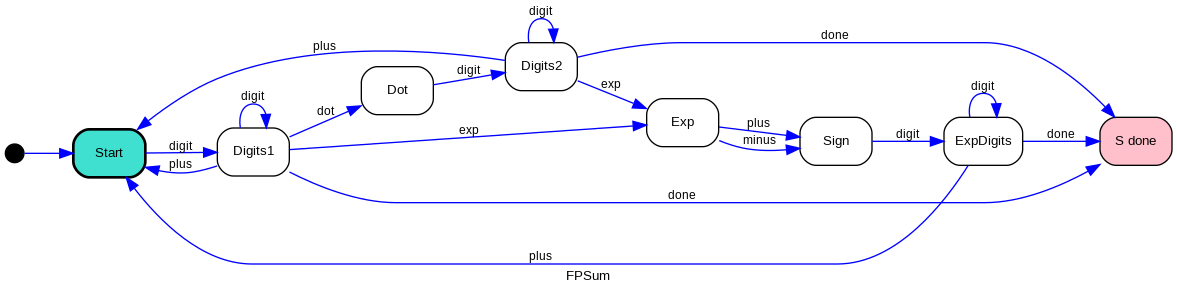
\includegraphics[scale=0.25]{fp_sum_expr.png}

    Example: \verb!123.45+60e+3+123.45e-67+12!
\end{frame}

\begin{frame}[fragile]{Measurement: State machine implementation methods}

    Compare:
\vspace{1cm}
\begin{itemize}
    \item Use existing \verb!python-statemachine! library
    \item Use \verb!for! loop with a \verb!match! statement
    \item Use a regular expression: \\
        \verb!r'\d+(\.\d+)?(e[+-]\d+)?(\+\d+(\.\d+)?(e[+-]\d+)?)*\$'!
    \item Use gotos for transition between states
\end{itemize}
\vspace{1cm}
    Using valid 30,000 character strings

\end{frame}
%\begin{frame}[fragile]{Measurement: How fast is using goto?}
%%\includepdf[pages={1}, fitpaper=false]{oddeven.pdf}
%%\includegraphics[scale=0.5]{oddeven.pdf}
%
%\begin{itemize}
%\item Function-based state machine within a class
%\item Goto-based state machine within a function
%\item \verb!while! loop in plain code
%\end{itemize}
%
%The \emph{even} state breaks at n = 100000000
%
%Python 3.3.1 on Linux VM
%\end{frame}

\begin{frame}[fragile]{Measurement: results}
    \begin{table}[]
\begin{tabular}{l|r|r}
 Method & Recognition time & Slowdown \\
 \hline
python-statemachine & 504ms & 180x  \\
for-loop with match & 21ms & 7.5x  \\
regular expression & 3.1ms & 1.1x  \\
goto & 2.8ms & 1x
\end{tabular}
\end{table}
\end{frame}

%\begin{frame}[fragile]{Performance (function-based state machine)}

%%Function-based state machine
%\begin{minted}{python}
%class state_machine:
%    def even_state(self):
%        ...
%        return self.odd_state
%    def odd_state(self):
%        ...
%        return self.even_state
%    def go():
%        state = self.even_state
%        while state:
%            state = state()
%\end{minted}
%\alert{35.0 seconds}
%\end{frame}

%
%\begin{frame}[fragile]{Performance (plain while loop)}
%\begin{minted}{python}
%n = 0
%while n != limit:
%    n += 1         # even -> odd
%    n += 1         # odd -> even
%\end{minted}
%\alert{11.5 seconds}
%\end{frame}
%
%\begin{frame}[fragile]{Performance (goto-based state machine)}
%%\vspace{-1cm}
%\begin{minted}{python}
%@goto
%def goto_state_machine(limit):
%    n = 0
%
%    label .state_even  ### even_state
%    if n == limit:
%        return
%    n += 1
%    goto .state_odd
%    ################
%    label .state_odd   ### odd_state
%    n += 1
%    goto .state_even
%\end{minted}
%\pause
%\alert{7.2 seconds!}  (over 4 seconds \emph{faster} than a \verb!while! loop!)
%
%\pause
%But... \verb!while! loop \emph{inside} function: \alert{7.1 seconds.} :-(
%\end{frame}

\begin{frame}[fragile]{Musings}

\begin{itemize}
    \item Bytecode rewriting is powerful
    \item Non-standard: CPython only
    \item Fast but fragile: Bytecode can change between python versions
    \item Historic re-enactment and fast state machines
    \item Don't use in production!
\end{itemize}
Questions?% (e.g. What about a \verb!comefrom! statement?)
%\begin{itemize}
%\item Remove some restrictions where sensible.
%\item pypi or something...
%\item \verb!comefrom! statement
%\item Computed \verb!goto!
%\end{itemize}

\end{frame}

\end{document}
